\section{Data Visualization and Insights}\label{sec:data_visualization}

Now that our probe data and SST tool are integrated, we can use various visualization tools to analyze our data and present statistical insights and valuable information based on the requirements. There are numerous tools and services available for data visualization. We have already discussed some key visualization tools in~\autoref{sec:component-visualizer}. In this section, we provide a brief summary of the visualization tools used in this report.

\subsection{Neo4j Desktop}
Neo4j provides its own application, \textit{Neo4j Desktop}\footnote{\url{https://neo4j.com/download}}, to visualize data stored in a Neo4j database. Users can connect to both local and remote Neo4j servers. The application includes several tools for visualizing different types of data.

One key tool is \textit{Neo4j Browser}\footnote{\url{https://neo4j.com/docs/browser-manual/current/}}, a web-based query tool for running Cypher queries. Another is \textit{Neo4j Bloom}\footnote{\url{https://neo4j.com/product/bloom/}}, which allows users to explore graph data interactively.

% In addition to these, other tools include the \textit{Graph Data Science (GDS)} Library, which provides implementations of graph algorithms\footnote{\url{https://neo4j.com/docs/gds/}}, and the \textit{ETL Tool}, which migrates relational data into Neo4j\footnote{\url{https://neo4j.com/labs/etl-tool/1.5.0/}}.

\subsection{Tableau}
\textit{Tableau is a leading data visualization tool used for data analysis and business intelligence}~\citep{biswal2024visualization}. It is known for its ease of use, compatibility with diverse data sources, and ability to create interactive dashboards that enhance data exploration and decision-making\footnote{\url{https://www.tableau.com/}}. One of the key reasons for choosing Tableau is its flexibility in handling various types of data while offering intuitive visualizations.

Since our SST tool stores data in a Neo4j database, Tableau provides a way to integrate with Neo4j, allowing real-time data capture and analysis. Additionally, it supports visualizing relationships between data points, aligning with Neo4j's graph-based structure.

\subsection{Tool Selection and Justification}

In this report, we will use Tableau and Neo4j Desktop to demonstrate the functionality of the probes and SST framework and validate our scenarios. Neo4j Desktop will be used for managing and visualizing graph-based data, while Tableau, which provides a way to connect directly with the Neo4j database, will assist in creating insightful visual representations. Using these tools, we aim to illustrate the framework's workings and ensure proper scenario validation.


% \begin{figure}[H]
%     \centering
%     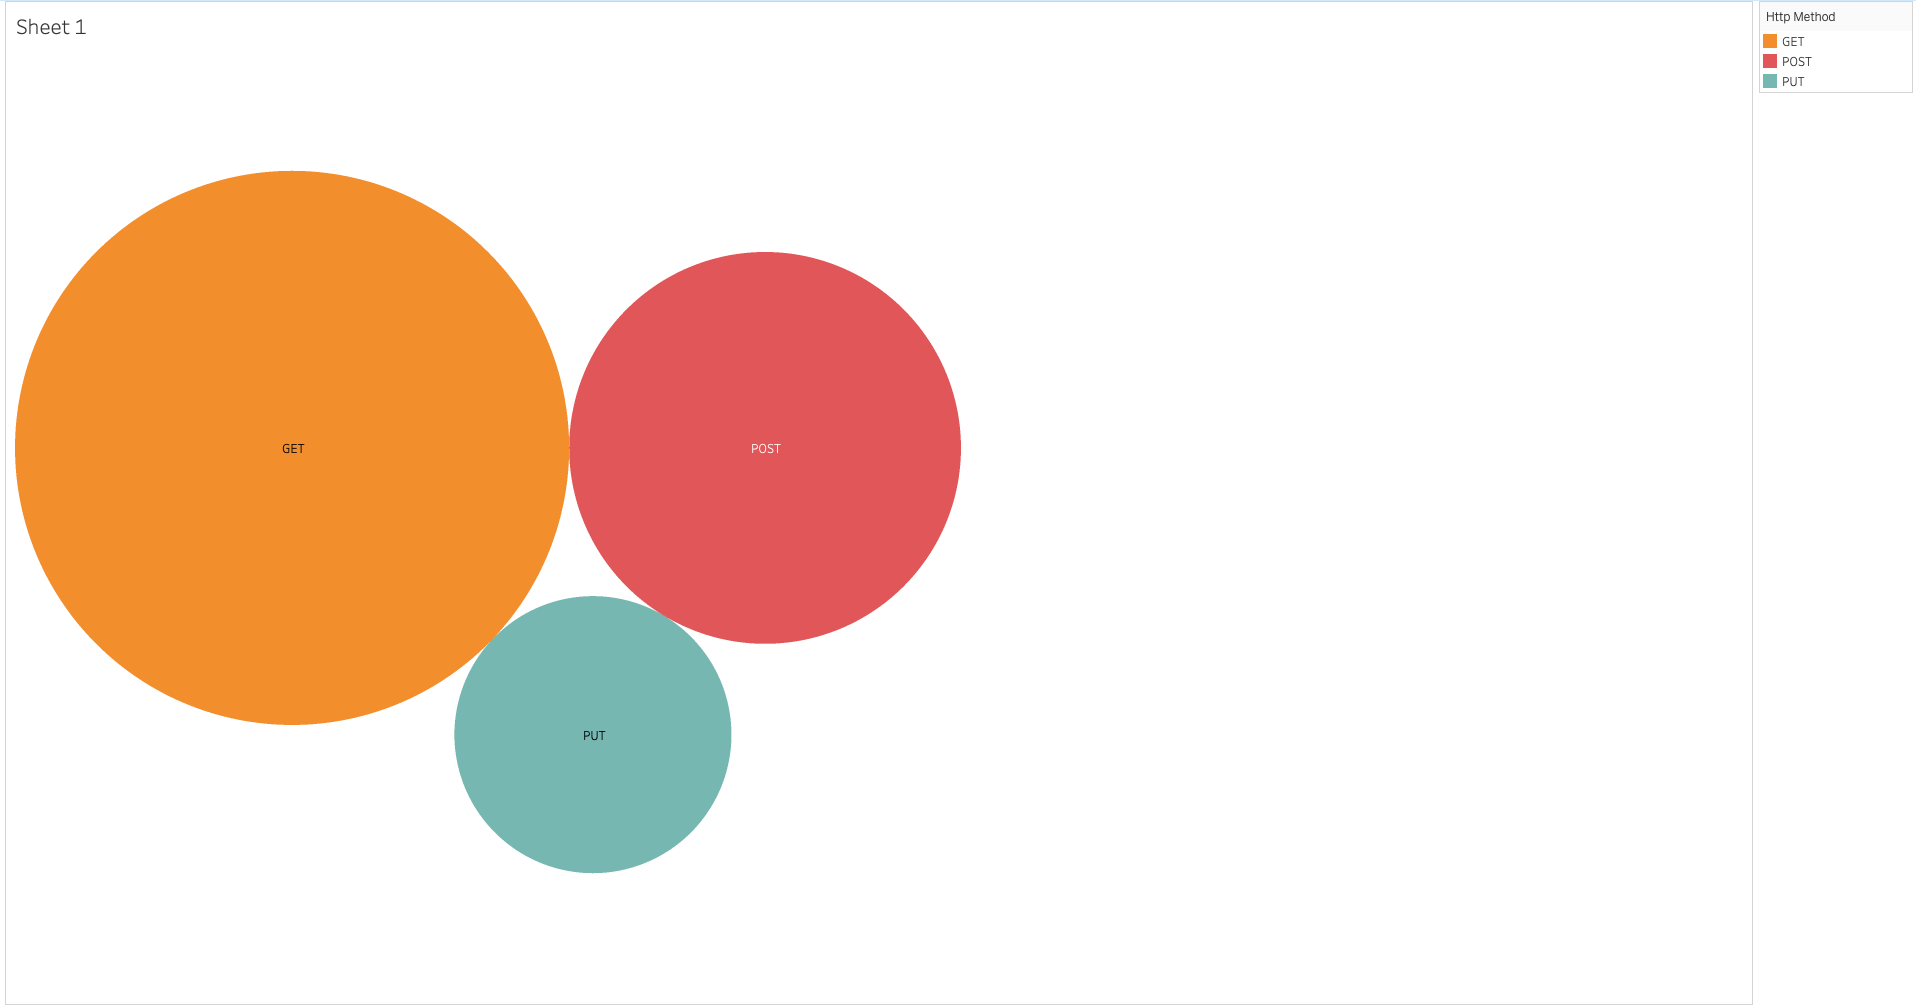
\includegraphics[width=1\textwidth]{figures/tableau_1.png}
%     \caption{REST API requests dominance}
%     \label{fig:tableau}
% \end{figure}


% For example, if we want to identify the dominance request types in our microservices, we can leverage the data stored in Neo4j (our SST tool) and connect it to a visualization platform.

% To demonstrate this, we will use Tableau as our visualizer tool. By linking Tableau with Neo4j, we can create interactive charts and dashboards to better understand request patterns, trends, and system behavior. This approach will help us make informed decisions based on clear and structured data representation.

% \begin{figure}[H]
%     \centering
%     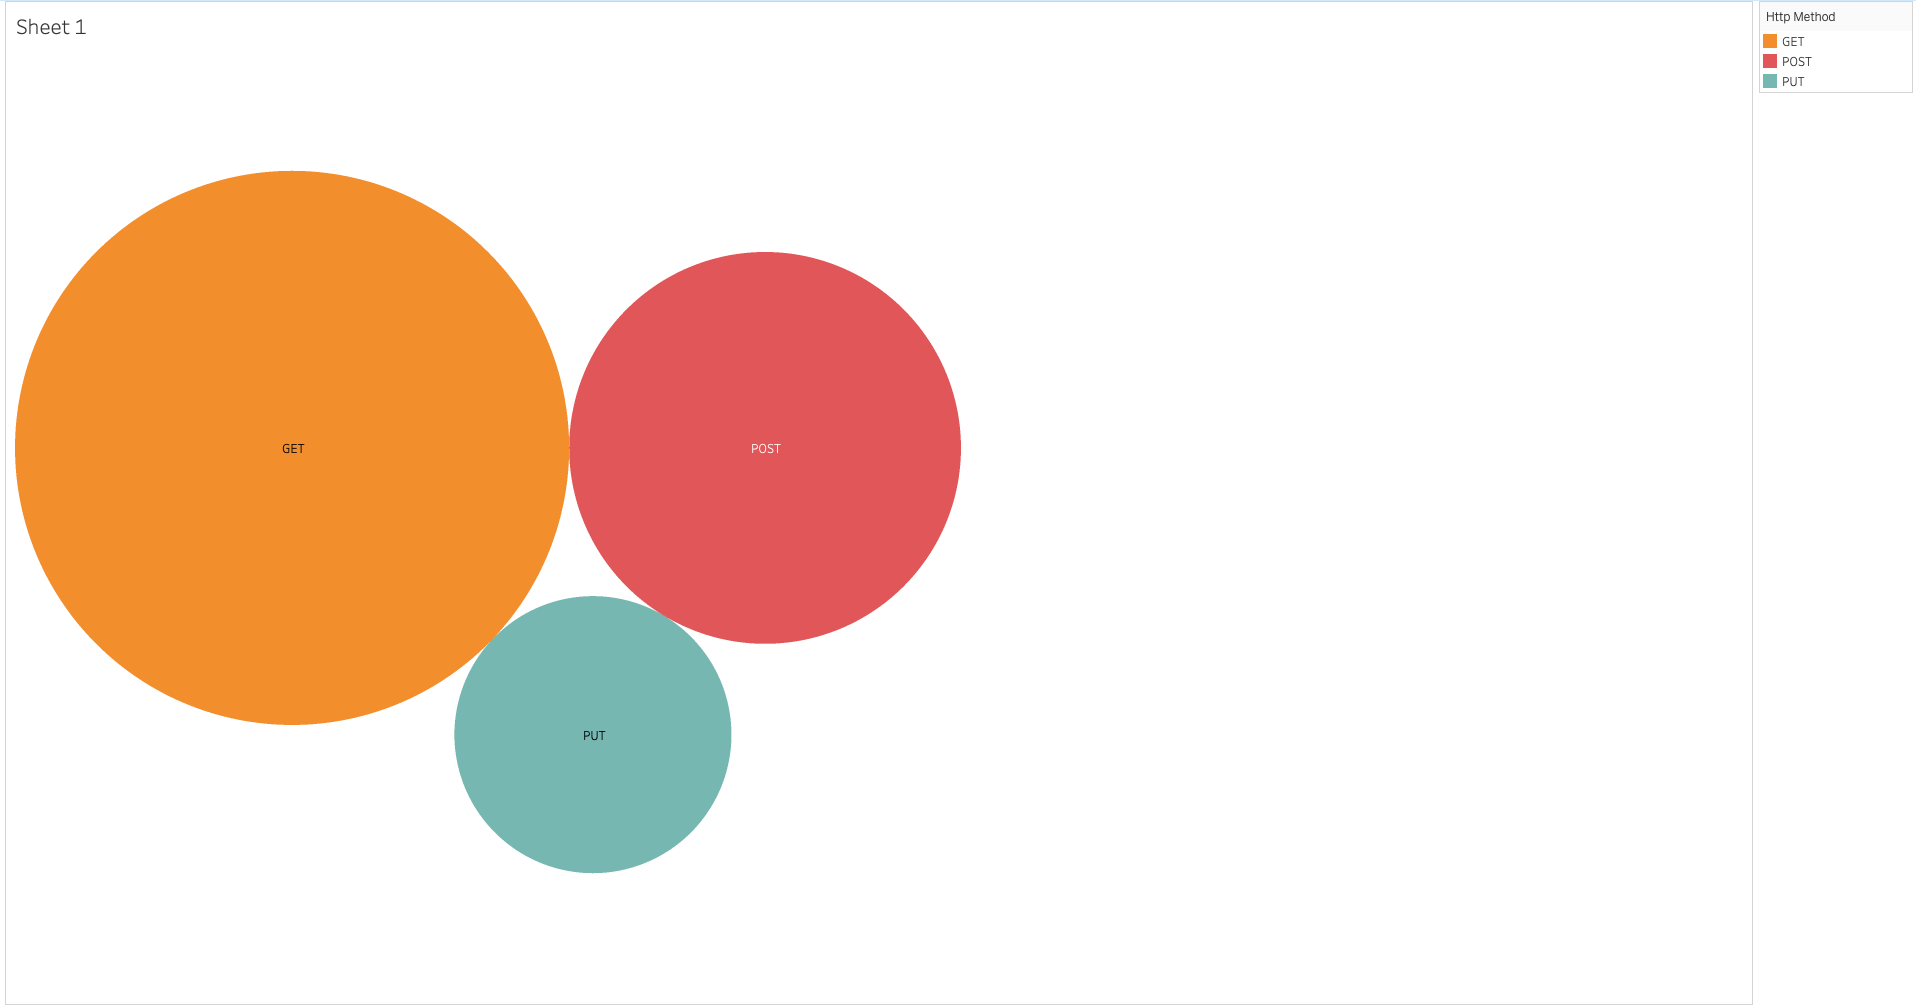
\includegraphics[width=1\textwidth]{figures/tableau_1.png}
%     \caption{REST API requests dominance}
%     \label{fig:tableau}
% \end{figure}